\documentclass[10.5pt,notitlepage]{article}
\usepackage[utf8]{inputenc}
\usepackage{amsthm}
\usepackage{amsmath}
\usepackage{amsfonts}
\usepackage{mathtools}
\usepackage{amsmath,amssymb}       
\usepackage{enumitem}   
\usepackage{enumerate}
\usepackage{verbatim} 
\usepackage{bbm}
\usepackage{hyperref}
\usepackage{booktabs}
\renewcommand{\qedsymbol}{$\blacksquare$}
\usepackage{makecell}
\usepackage[spanish]{babel}
\decimalpoint
\usepackage[letterpaper]{geometry}
\usepackage{mathrsfs}
\newenvironment{solucion}
  {\begin{proof}[Solución]}
  {\end{proof}}
\pagestyle{plain}
\usepackage{pdflscape}
\usepackage[table, dvipsnames]{xcolor}
\usepackage{longtable}
\usepackage{tikz}
\def\checkmark{\tikz\fill[scale=0.4](0,.35) -- (.25,0) -- (1,.7) -- (.25,.15) -- cycle;} 
\usepackage[bottom]{footmisc}
\usepackage{hyperref}
\usepackage{float}
\usepackage[utf8]{inputenc}
\usepackage{bbm}
\usepackage[backend=biber,style=apa]{biblatex}
\usepackage{csquotes}
\DeclareLanguageMapping{spanish}{spanish-apa}
\urlstyle{same}
\addbibresource{refer.bib}
\usepackage{etoolbox}
\patchcmd{\thebibliography}{\section*{\refname}}{}{}{}
\usepackage{placeins}
\newcommand{\pp}{\mathbb{P}}
\newcommand{\BB}{\mathcal{B}}
\newcommand{\RR}{\mathbb{R}}
\newcommand{\Ff}{\mathcal{F}}
\newcommand{\Jj}{\mathcal{J}}
\newcommand{\Cc}{\mathcal{C}}
\newcommand{\oo}{\varnothing}
\newcommand{\ee}{\varepsilon}
\newcommand{\EE}{\mathbb{E}}
\newcommand{\NN}{\mathbb{N}}
\newcommand{\PP}{\mathcal{P}}
\newcommand{\LL}{\mathrm{L}}
\newcommand{\XX}{\mathbf{X}}
\newcommand{\xx}{\mathbf{x}}
\DeclareMathOperator{\Tr}{Tr}
\newcommand{\abs}[1]{\left\lvert #1 \right\rvert}
\newcommand{\norm}[1]{\left\| #1 \right\|}
\newcommand{\inner}[1]{\left\langle #1 \right\rangle}
\newcommand{\corch}[1]{\left[ #1 \right]}
\newcommand{\kis}[1]{\left\{ #1 \right\}}
\newcommand{\pare}[1]{\left( #1 \right)}

\theoremstyle{plain}

\newtheorem{thm}{Teorema}[section] % reset theorem numbering for each chapter
\newtheorem{defn}[thm]{Definición} % definition numbers are dependent on theorem numbers
\newtheorem{lem}[thm]{Lema} % same for example numbers
\newtheorem{remarkex}{Observación}
\newenvironment{rem}
  {\pushQED{\qed}\renewcommand{\qedsymbol}{$\triangle$}\remarkex}
  {\popQED\endremarkex}

\usepackage{geometry}
\usepackage{mathtools}
\usepackage{enumitem}
\usepackage{framed}
\usepackage{amsthm}
\usepackage{thmtools}
\usepackage{etoolbox}
\usepackage{fancybox}

\newenvironment{myleftbar}{%
\def\FrameCommand{\hspace{0.6em}\vrule width 2pt\hspace{0.6em}}%
\MakeFramed{\advance\hsize-\width \FrameRestore}}%
{\endMakeFramed}
\declaretheoremstyle[
spaceabove=6pt,
spacebelow=6pt
headfont=\normalfont\bfseries,
headpunct={} ,
headformat={\cornersize*{2pt}\ovalbox{\NAME~\NUMBER\ifstrequal{\NOTE}{}{\relax}{\NOTE}:}},
bodyfont=\normalfont,
]{exobreak}

\declaretheorem[style=exobreak, name=Ejercicio,%
postheadhook=\leavevmode\myleftbar, %
prefoothook = \endmyleftbar]{exo}
\usepackage{graphicx}
\graphicspath{ {images/} }
\title{Parcial 3: Modelos Estadísticos I.}

\author{Rojas Gutiérrez Rodolfo Emmanuel}
\begin{document}

\maketitle

\setcounter{exo}{0}
\begin{exo}

\end{exo}
\begin{rem}
A lo largo de este ejercicio, \(devres\) denotará a la deviance residual y \(df\) a los grados de libertad de la misma, \(d1\) representa a la dosis de radiación, \(d2\) a la dosis de radiación al cuadrado y \(d3\) a la respectiva dosis de radiación al cubo.
\end{rem}
\begin{solucion}
\textit{1} Como se están considerando proporciones se hará uso de un GLM binomial. Para el modelo 1), se considero el GLM binimial con componente sistemático:\footnote{Donde \(\pi\) denota a la probabilidad de morir por leucemia, en lugar de por algún otro cáncer, dado que se estuvo expuesto a cierta dosis de radiación. }
\begin{equation}\label{Mod1}
    g(\pi) = \beta_0 + \beta_{1}d1,
\end{equation}
cabe destacar que se uso la liga logit, con lo que se obtuvieron las estimaciones en \(R\) presentadas en la figura \ref{fig1}.
\begin{figure}[htb]
    \centering
    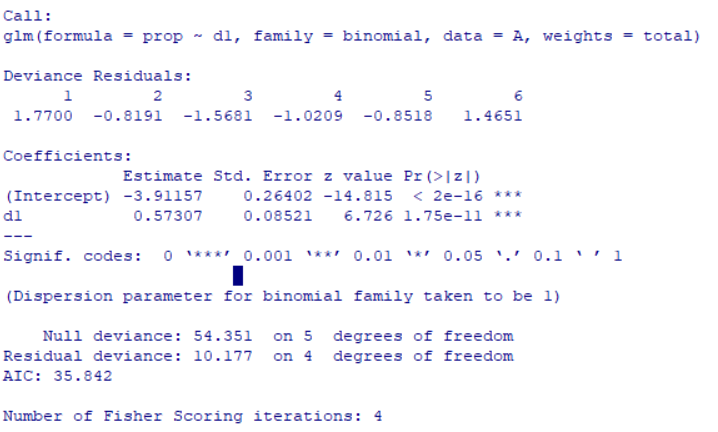
\includegraphics[scale = 0.5]{fit1Im.png}
    \caption{Estimaciones modelo \eqref{Mod1}.}
    \label{fig1}
\end{figure}
Como puede verse, bajo los estadísticos de Wald se ha obtenido que todos los coeficientes de este modelo, resultan significativamente distintos de cero, bajo un nivel de significancia del \(5\%\). Además, se tiene que este modelo cuenta con 
\begin{equation}\label{AIC1}
    AIC = 35.842, \ devres = 10.177 \text{ con } df = 4.  
\end{equation}
Dado que la deviance residual no es mucho mayor a sus grados de libertad, no se considerará necesario ajustar un modelo que consideré sobredispersión en los datos. Por último, se deja en la parte izquierda de la figura \ref{figtodas}, una gráfica de los valores ajustados por este modelo, más intervalos de confianza al \(95\%\) en lineas azules y observaciones en puntos rojos, podemos ver que el ajuste no es óptimo, parece que nos esta haciendo falta considerar cierta curvatura en los datos, lo cual se verá a continuación. Pese a ello, como ya se comento, los coeficientes son todos significativos, por lo que, este modelo puede ser un buen punto de partida para buscar una mejor alternativa, el \(AIC\) se usará más adelante para la selección del modelo. \\



\textit{2} Para el modelo 2), se considero el GLM binimial con componente sistemático:
\begin{equation}\label{Mod2}
    g(\pi) = \beta_0 + \beta_{1}d1+\beta_2 d2,
\end{equation}
cabe destacar que se uso la liga logit, con lo que se obtuvieron las estimaciones en \(R\) presentadas en la figura \ref{fig2}.
\begin{figure}[htb]
    \centering
    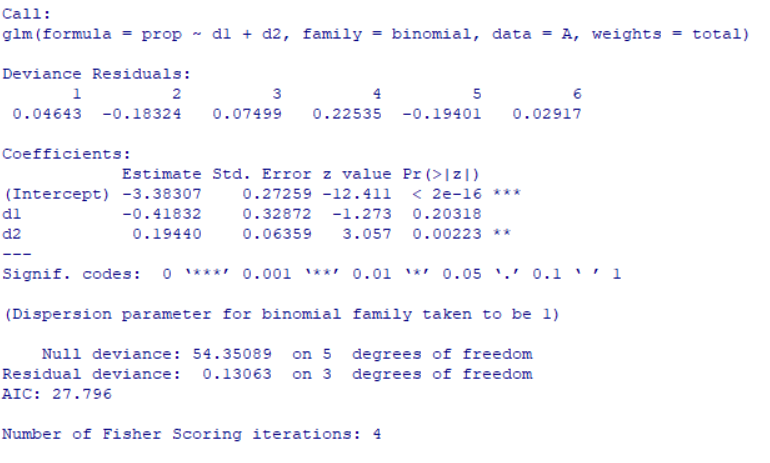
\includegraphics[scale = 0.5]{fit2Im.png}
    \caption{Estimaciones modelo \eqref{Mod2}.}
    \label{fig2}
\end{figure}
Observe que, en este modelo el coeficiente que pre-multiplica a la variable explicativa \(d1\), resulta ser no significativo bajo un nivel de significancia del \(5\%\), sin embargo, los demás coeficientes si resultan ser significativos bajo el nivel mencionado. Adicionalmente, se tiene que este modelo cuenta con: 
\begin{equation}\label{AIC2}
    AIC = 27.796, \ devres = 0.13063 \text{ con } df = 3.  
\end{equation}
Aquí, la deviance residual es muy pequeña mucho menor que sus grados de libertad, lo que nos habla de un buen ajuste del modelo.\footnote{Aunque no puede descartarse un sobreajuste, debido a que al menos un coeficiente no es significativo}. Por otro lado, en la parte de en medio de la figura \ref{figtodas}, se puede observar una gráfica de los valores ajustados por este modelo, más intervalos de confianza al \(95\%\) en lineas azules y observaciones en puntos rojos, vemos que la curvatura que hacía falta considerar en el modelo \eqref{Mod1} parece haber desaparecido, sin embargo, pareciera haber cierto grado de sobre-ajuste del modelo. \\ 

\textit{3} Para el modelo 3), se considero el GLM binimial con componente sistemático:
\begin{equation}\label{Mod3}
    g(\pi) = \beta_0 + \beta_{1}d1+\beta_2 d2 + \beta_{3}d3,
\end{equation}
cabe destacar que se uso la liga logit, con lo que se obtuvieron las estimaciones en \(R\) presentadas en la figura \ref{fig3}.
\begin{figure}[htb]
    \centering
    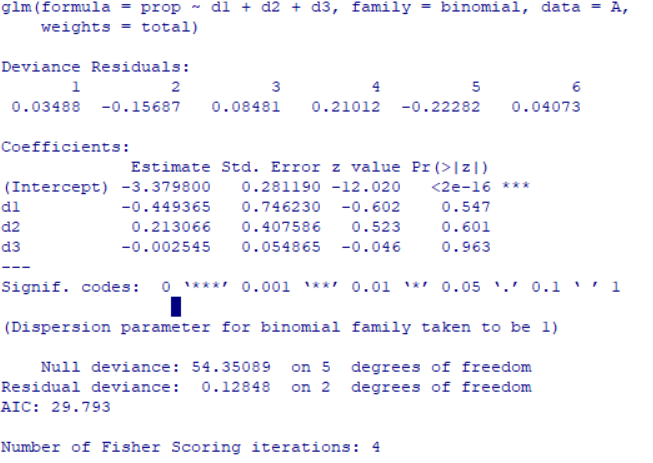
\includegraphics[scale = 0.5]{fit3Im.png}
    \caption{Estimaciones modelo \eqref{Mod3}.}
    \label{fig3}
\end{figure}
Aquí, parece que ya estamos utilizando demasiadas covariables en el modelo, puesto que ninguna de ellas resulta ser significativamente distinta de \(0\), bajo un nivel de significancia del \(5\%\), pese a que en los modelos anteriores, que consideraban una cantidad menor de covariables si que lo eran. Por otro lado, este modelo  cuenta con: 
\begin{equation}\label{AIC3}
    AIC = 29.793, \ devres = 0.12848 \text{ con } df = 2.  
\end{equation}
Vemos que nuevamente la deviance residual es mucho menor a sus grados de libertad, inclusive aún, más que en el modelo considerado en el inciso 2. Por último, se deja en la parte derecha de la figura \ref{figtodas} una gráfica de los valores ajustados por este modelo, más intervalos de confianza al \(95\%\) en lineas azules y observaciones en puntos rojos. En está gráfica no queda duda del nivel de sobreajuste por parte de este modelo. \\ 

\begin{figure}[htb]
    \centering
    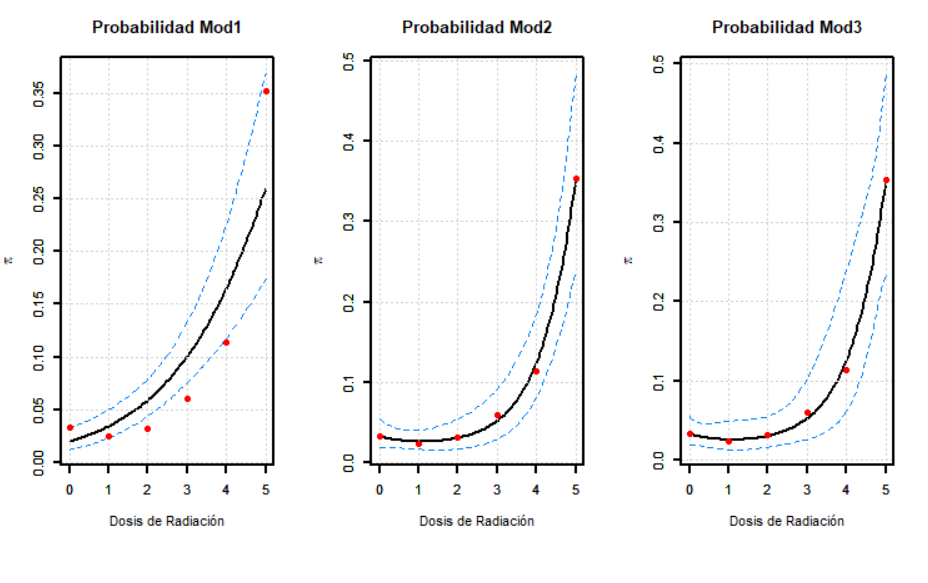
\includegraphics[scale = 0.5]{Im1.png}
    \caption{Valores ajustados por los tres modelos, más intervalos de confianza al \(95\%\) en lineas azules y observaciones en puntos rojos.}
    \label{figtodas}
\end{figure}

\textit{4} De los tres modelos comparados en los incisos anteriores, claramente el mejor resulta ser el modelo \eqref{Mod2} considerado en el inciso 2), ya que el nivel de ajuste en las gráficas parece ser adecuado y cuenta con el menor \(AIC\) de los tres modelos considerados, sin embargo, cuenta con un ligero problema, uno de sus coeficientes resulta no ser significativamente distinto de cero, bajo un nivel de significancia del \(5\%\), en este inciso buscaremos optimizar dicho modelo, de ser posible. Primeramente, para corroborar que las variables \(d1\) y \(d2\) son las que más información aportan a este modelo, se deja el siguiente análisis anova: 

\begin{figure}[htb]
    \centering
    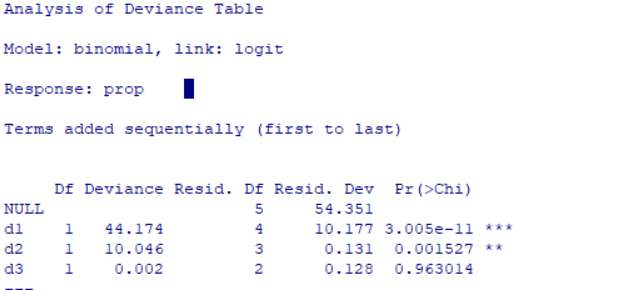
\includegraphics[scale = 0.5]{AnovaIm.png}
    \caption{Análisis anova.}
    \label{figtodas}
\end{figure}
En este análisis observamos que el agregar el predictor \(d3\) al modelo realmente no resulta relevante, dado que el \(p\)-valor de la prueba en el que no se considera este coeficiente es bastante alto, prácticamente cercano a \(1\). Por otro lado, los otros dos coeficientes resultan bastante significativos, bajo un nivel de significancia del \(5\%\). Puesto que ya ajustamos, el modelo que considera solo a \(d1\) y el que considera a \(d2\) y a \(d1\), donde como ya se mencionó fue claramente superior el modelo que considerá a ambas covariables, veremos que tal resulta el ajuste del modelo que únicamente considera a \(d2\), es decir el \(glm\) binomial con componente sistemático: 
\begin{equation}\label{Mod4}
    g(\pi) = \beta_0 +\beta_2 d2,
\end{equation}
cabe destacar que se uso la liga logit, con lo que se obtuvieron las estimaciones en \(R\) presentadas en la figura \ref{fig4}.
\begin{figure}[htb]
    \centering
    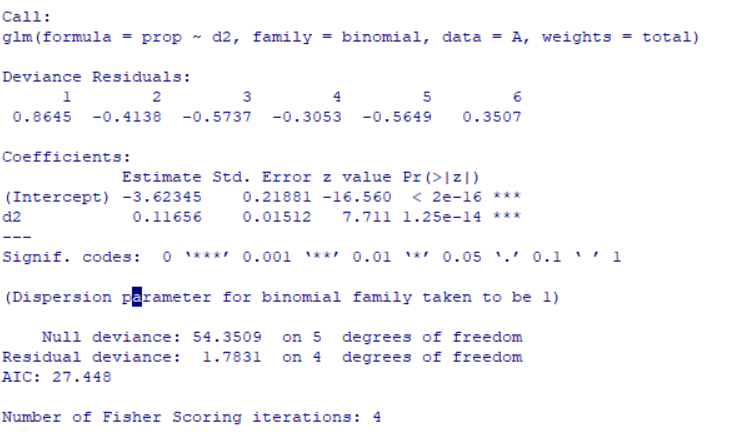
\includegraphics[scale = 0.5]{fit4Im.png}
    \caption{Estimaciones modelo \eqref{Mod4}.}
    \label{fig4}
\end{figure}
Observe que, todos los coeficientes de este modelo resultan ser significativamente distintos de cero, bajo un nivel de significancia del \(5\%\). Además, este modelo cuenta con:
\begin{equation}\label{AIC4}
    AIC = 27.448, \ devres = 1.7831 \text{ con } df = 4.  
\end{equation}
Puede observar que la deviance residual es menor que sus grados de libertad, sin llegar a ser excesivamente pequeña como en los casos de los modelos en \eqref{Mod3} y \eqref{Mod2}, lo que es un buen primer indicio de un ajuste más que razonable del modelo.\footnote{Esto además nos vuelve a indicar la no existencia de sobredispersion}
Por otro lado, en la figura \ref{figtod}, puede observar  una gráfica de los valores ajustados por este modelo, más intervalos de confianza al \(95\%\) en lineas azules y observaciones en puntos rojos. En la misma, se ve un ajuste más que razonable, sin parecer que el modelo trata de pasar por todas las observaciones en el mismo, es decir no parece existir sobre ajuste, como en los modelos en \eqref{Mod2} y \eqref{Mod3}. Más aún, cuenta con un \(AIC\) de \(27.488\), lo que es menor que el hasta ahora mejor modelo, modelo \eqref{Mod2} con un AIC de acuerdo con \eqref{AIC2} de \(27.796\). Así, se elige este como el mejor modelo posible, con las covariables dadas y sus derivados. 
\begin{figure}[htb]
    \centering
    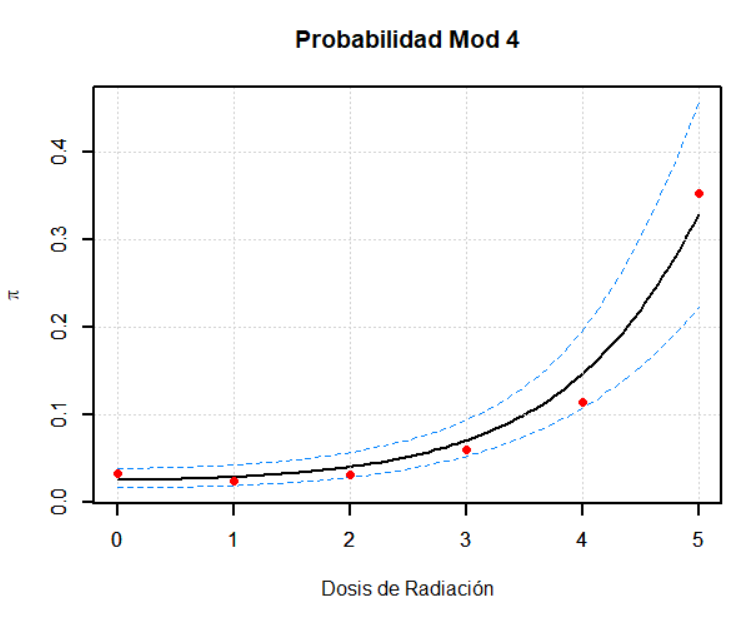
\includegraphics[scale = 0.5]{Im2.png}
    \caption{Valores ajustados por el modelo \eqref{Mod4}, más intervalos de confianza al \(95\%\) en lineas azules y observaciones en puntos rojos.}
    \label{figtod}
\end{figure}
\end{solucion}

\begin{exo}

\end{exo}
\begin{solucion}
\textbf{a)} Para este inciso se considerará el ajuste del \(GLM\) poisson, con componente sistemático: 
\begin{equation}\label{Mod10}
    g(\mu) = \beta_0 + \beta_1 X. 
\end{equation}
donde \(\mu = E[Y|X]\) y \(g\) es la liga logarítmica. Haciendo uso de \(R\) se obtuvieron las estimaciones de los coeficientes presentadas en la figura \ref{fig10}: 
\begin{figure}[htb]
    \centering
    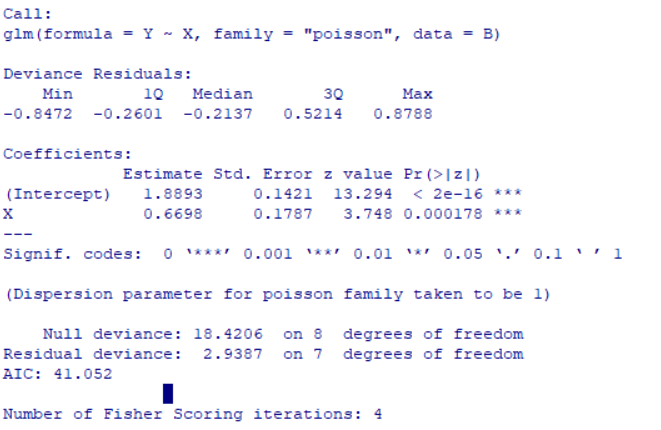
\includegraphics[scale = 0.5]{Ej2fit1.png}
    \caption{Estimaciones modelo \eqref{Mod10}.}
    \label{fig10}
\end{figure}
Como puede notarse, todos los coeficientes de este modelo resultan significativamente distintos de cero, bajo un nivel de significancia del \(5\%\). Además, este modelo cuenta  con: 
\begin{equation}\label{AIC10}
    AIC = 41.052, \ devres = 2.9387 \text{ con } df = 7.  
\end{equation}
Se nota que la deviance residual resulta bastante más chica que sus grados de libertad, lo que nos habla de la no existencia de sobredispersión,\footnote{Por lo que no habrá que considerar un modelo que considere este aspecto.} además, dado que la deviance residual del modelo es muy pequeña, se puede hablar de un buen ajuste del modelo. Esto último, puede corroborarse en la gráfica a la izquierda de la figura \ref{figtodas2}, donde se aprecia una gráfica de los valores ajustados por este modelo, más intervalos de confianza al \(95\%\) en lineas azules y observaciones en puntos rojos, además, no pareciera existir sobreajuste al menos visualmente. El criterio de Akaike será utilizado mas adelante, para comparar este modelo con el que será ajustado en el siguiente inciso. \\ 

\textbf{b)} Para este inciso se considerará el ajuste del \(GLM\) poisson, con componente sistemático: 
\begin{equation}\label{Mod11}
    g(\mu) = \beta_0 + \beta_1 X. 
\end{equation}
donde \(\mu = E[Y|X]\) y \(g\) es la liga identidad. Para el que, nuevamente haciendo uso de \(R\), se obtuvieron las estimaciones presentadas en la figura \ref{fig11}. 
\begin{figure}[htb]
    \centering
    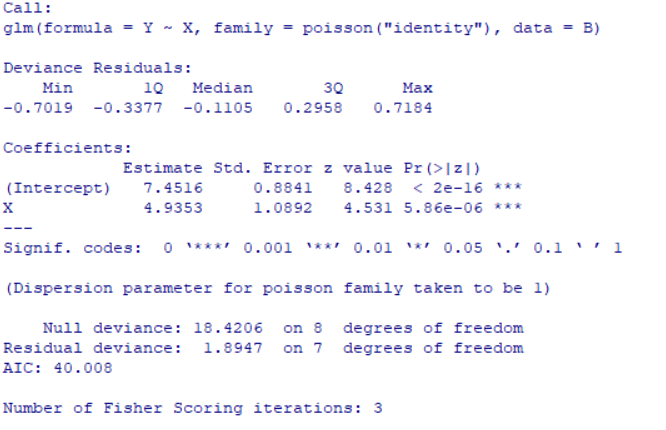
\includegraphics[scale = 0.5]{Ej2fit2.png}
    \caption{Estimaciones modelo \eqref{Mod11}.}
    \label{fig11}
\end{figure}
Note que, al igual que en el modelo anterior todos los coeficientes resultan significativamente distintos de cero, bajo un nivel de significancia del \(5\%\), lo que es una señal inequivoca de un buen ajuste del modelo. Adicionalmente, se puede ver que este modelo cuenta con: 
\begin{equation}\label{AIC11}
    AIC = 40.008, \ devres = 1.8947 \text{ con } df = 7.  
\end{equation}
Nuevamente, se desataca que al igual que en el modelo anterior, la deviance residual resulta mucho menor a sus grados de libertad, además de que, no resulta excesivamente lejana de cero, por lo que, se tiene otro buen indicativo del ajuste del modelo. Finalmente, y como ya es costumbre se deja en la parte derecha de la figura \ref{figtodas2}, una gráfica de los valores ajustados por este modelo, más intervalos de confianza al \(95\%\) en lineas azules y observaciones en puntos rojos. Donde, al igual que en el caso anterior se ve en general un ajuste bastante razonable a los datos observados. Nuevamente, el \(AIC\) nos será de utilidad en los siguientes incisos.\\ 
\begin{figure}[htb]
    \centering
    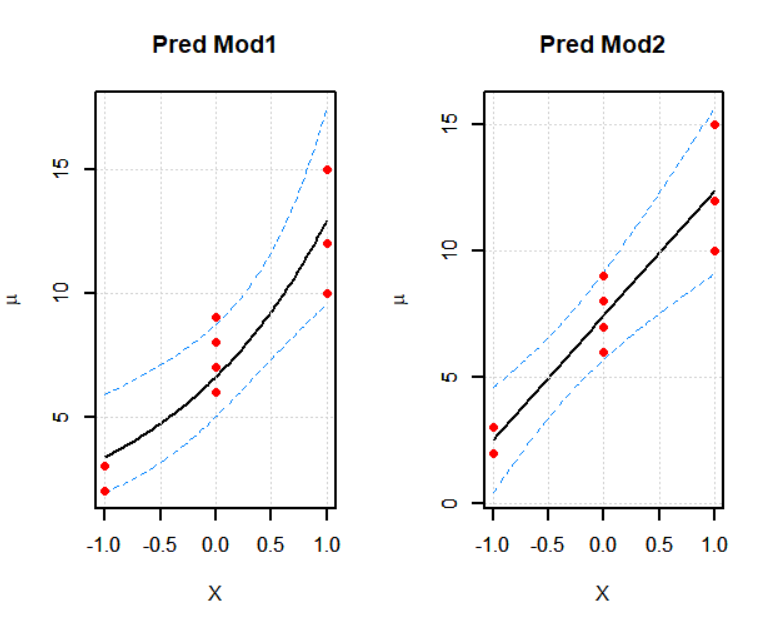
\includegraphics[scale = 0.5]{Ej2Im1.png}
    \caption{Valores ajustados por los dos modelos, más intervalos de confianza al \(95\%\) en lineas azules y observaciones en puntos rojos.}
    \label{figtodas2}
\end{figure}

\textit{c) y d)} Bajo los dos modelos analizados en los incisos anteriores, se observo un ajuste bastante similar a través de los cálculos realizados, ambos cuentan con coeficientes significativamente distindos de cero, una deviance residual pequeña y mucho menor a sus grados de liberta e incluso poseen \(AIC\) muy parecidos: 
\begin{align}
    AIC \text{ del modelo en \eqref{Mod10}}: 41.052, \nonumber\\ 
    AIC \text{ del modelo en \eqref{Mod11}}: 40.008 \label{AICC}. 
\end{align}
Además, observando las gráficas en \eqref{figtodas2}, nos percatamos de que visualmente el ajuste es también similar, salvo la evidente curvatura añadida por la liga logarítmica, tenemos un comportamiento similar en los intervalos de confianza, (son mas anchos hacía los extremos y más cerrads hacia el centro), y el mismo patrón creciente en las predicciones, por lo que, se decidió hacer uso de los residuales de cuantiles,\footnote{Ver \textcite{dunn_generalized_2018} capítulo 8  para una definición de los mismos.} los cuales deberían de distribuirse aproximadamente como normales estándar de estar siendo utilizado el glm correcto, con este idea en mente se construyeron las siguientes gráficas \(QQ\), presentadas en la figura \label{QQ} con los residuales de cuantiles de ambos modelos:
\begin{figure}[htb]
    \centering
    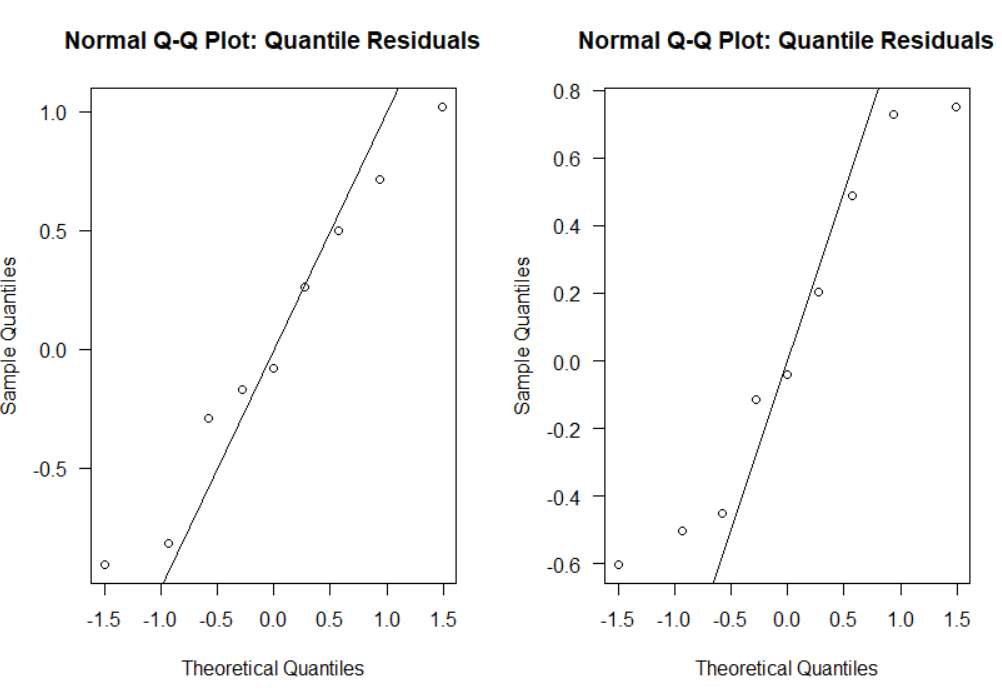
\includegraphics[scale = 0.5]{Ej2QQ.png}
    \caption{Gráficas \(QQ\) residuales de cuantiles, a la izquierda la del modelo en \eqref{Mod10} y  a la derecha la del modelo en \eqref{Mod11}.}
    \label{QQ}
\end{figure}
Como puede observarse, ambas gráficas presentan un ajuste razonable de los residuales hacia el centro de la distribución normal estándar, y ambas gráficas presentan problemas hacia las colas, por lo que, incluso bajo este criterio ambos modelos resultan muy similares. Por lo que, nos basaremos en el criterio menos subjetivo de todos estos para seleccionar al mejor de los dos, este es el \(AIC\), criterio bajo el cual puede comprobarse en \eqref{AICC}, es una mejor elección el modelo con liga identidad, ya que este posee el menor \(AIC\). Empíricamente esto puede verse en los gráficos de dispersión, presentados en la figura \ref{chafa}. 
\begin{figure}[htb]
    \centering
    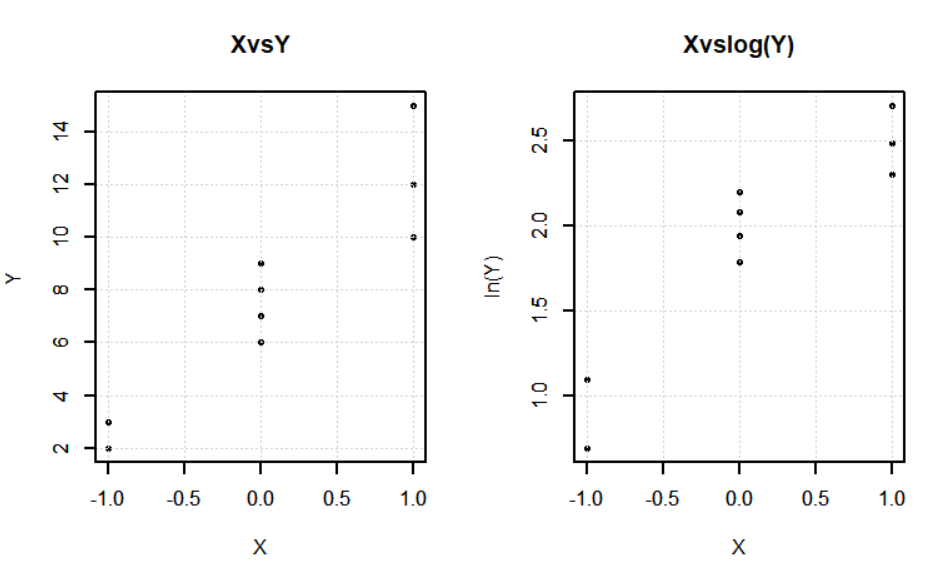
\includegraphics[scale = 0.5]{Ej2graficachafa.png}
    \caption{Gráfico de dispersión \(Y\) vs \(X\) a la izquierda, \(ln(Y)\) vs \(X\) a la derecha.}
    \label{chafa}
\end{figure}
En los cuales, se presenta un gráfico de dispersión \(Y\) vs \(X\) a la izquierda, \(log(Y)\) vs \(log(X)\) a la derecha. Aqui, se puede apreciar cierta relación lineal entre \(X\) e \(Y\), mientras que entre \(X\) y \(ln(Y)\) pareciera existir cierta curvatura en la relación que entre ambos variables, por lo que, si se quiere continuar usando dicha liga, podría considerarse meter algún termino polinomial de \(X\).
\end{solucion}

\section{Anexo}

 Como comentario final para el ejercicio 1, el modelo que considera únicamente a \(d3\) tiene por muy poco un menor\footnote{\(AIC = 26.19\)} \(AIC\) que el modelo elegido, sin embargo, parece tener cierto sobre ajuste, ver figura \ref{Sobreajus}, que era un propiedad no deseada desde el principio.
 \begin{figure}
     \centering
     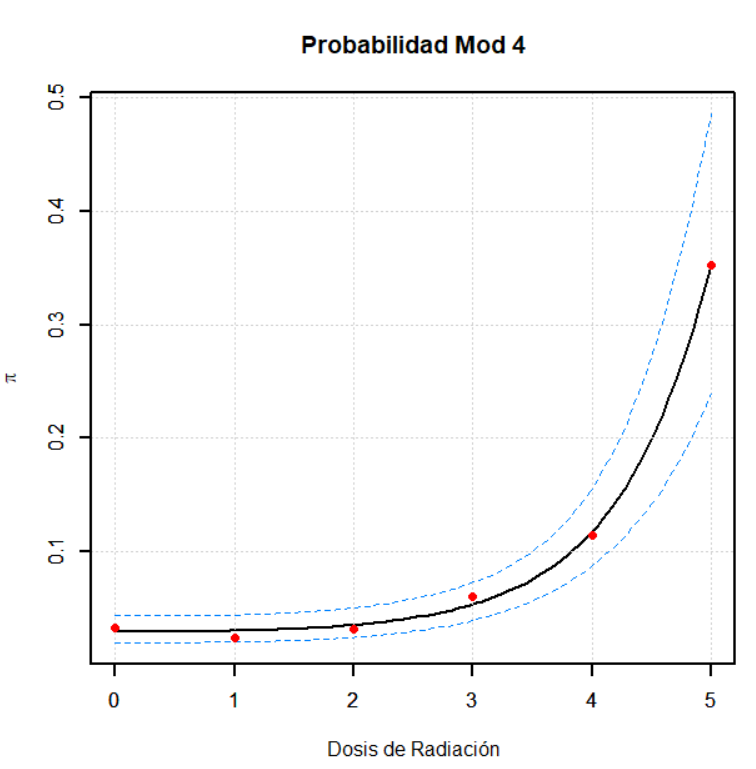
\includegraphics[scale = 0.5]{ModeloSObreajus.png}
     \caption{Modelo que solo considera a \(d3\)}
     \label{Sobreajus}
 \end{figure}

\newpage
\nocite{dunn_generalized_2018}
\printbibliography
\end{document}
